\chapter{An Augmented Quantum Threshold Scheme}
\label{ch:good-stuff}

In this section, we introduce our own idea to circumvent the no-cloning theorem, beginning with the following questions: What can we do if we were to start with two identical copies of a quantum state? What if we have $k$ copies? Can we create a scheme that circumvents the limitations imposed by the no-cloning theorem? If so, what schemes are realizable using this new formulation? In this section, we will explore the properties of such a scheme. We will call this an \textbf{augmented quantum threshold scheme}. Let us formalize this idea before exploring its properties below:

\theoremstyle{definition}
\begin{definition}{Augmented Quantum Threshold Scheme.}
    \label{defn:augmented-qts}
     This is a QTS that assumes that we begin with $k$ identical copies of a quantum state prepared in advance. As with the normal QTS, we need at least $t$ individuals to come together to recover the secret quantum state. We will denote an augmented QTS as $((t,n,k))$.
\end{definition}

\section{A Loose Upper Bound}

Based on the results presented in \sref{section:qss}, it would be most natural to begin our analysis of an augmented QTS by considering the consequences of the no-cloning theorem. Let us begin with the case where $k=2$. Then, we can extend \thmref{thm:qss-disjoint} in the following way:

\begin{theorem}
    \label{thm:three-authorized}
    In any valid $((t,n,2))$ scheme, any three authorized subsets cannot be pair-wise disjoint.
\end{theorem}

The proof for this theorem is very similar to that of \thmref{thm:qss-disjoint}. Here is that theorem generalized to $k$ copies for $k \geq 1$:

\begin{theorem}
    \label{thm:k-authorized}
    In any valid $((t,n,k))$ scheme, any $k+1$ authorized subsets cannot be pair-wise disjoint.
\end{theorem}

Using these two theorems, we can immediately propose an initial upper bound on the value of $n$ with respect to $t$ and $k$ in the case of threshold schemes. We give the case for $k=2$ as well as the more general case:

\begin{corollary}
	\label{cor:qts2}
	An augmented QTS of the form $((t,n, 2))$ can exist only if $t > \frac{n}{3}$, which is equivalent to $n \leq 3t-1$.
\end{corollary}

\begin{corollary}
	\label{cor:qtsk}
	An augmented QTS of the form $((t,n, k))$ can exist only if $t > \frac{n}{k+1}$, which is equivalent to $n \leq (k+1)t-1$.
\end{corollary}

Just as Theorems \ref{thm:three-authorized} and \ref{thm:k-authorized} extend \thmref{thm:qss-disjoint}, these Corollaries extend \corref{cor:qts}, and while they are a good start to our analysis, they only provide to us what schemes are not immediately ruled out by the no-cloning theorem. Figuring out methods of realizing these schemes is a different question, and that is what we consider in the following section.

\section{A Union of Access Structures Approach}
\label{sec:union-access-structures}

The simplest non-trivial case to implement is a $((2,4,2))$ scheme. Using two identical copies of a quantum state, we ask the following question: Is it possible to implement a scheme among four individuals such that only two or more people need to come together to recover the secret. The answer is yes.

To construct this scheme, we will use the following approach: we take the access structure that we want to implement and split it up into two smaller access structures, each of which are valid access structures, which means that on their own, they are monotone and satisfy the no-cloning theorem. By \thmref{thm:monotone-gamma}, we assume that there exists an implementation of a quantum secret sharing scheme that corresponds to our valid access structures, and we assign one copy to each of them. We will call this procedure the union of access structures approach.

Let the two copies of our quantum secret be $\ket{\psi_1}$ and $\ket{\psi_2}$, and let the participants be labeled $p_1, p_2, p_3, p_4$. \fref{fig:2-4-2} shows how we implement the scheme. Each vertex corresponds to one participant. The blue edges denote authorized subsets of size 2 that are a part of the access structure $\Gamma_1$ of $\ket{\psi_1}$. Red edges correspond to $\Gamma_2$, which is the access structure of $\ket{\psi_2}$.


\begin{figure}[H]
	\begin{center}
        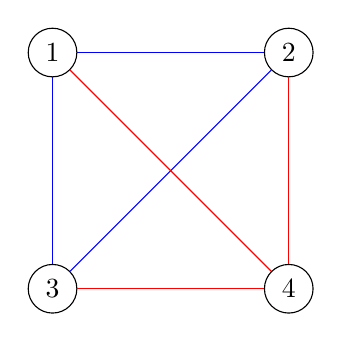
\begin{tikzpicture}[scale=3,auto=left,every node/.style={circle,draw,fill=white}]
          \node (n1) at (0,1) {1};
          \node (n2) at (1,1) {2};
          \node (n3) at (0,0) {3};
          \node (n4) at (1,0) {4};
          
          \draw [blue] (n1) -- (n2);
          \draw [blue] (n3) -- (n2);
          \draw [blue] (n1) -- (n3);
          \draw [red] (n1) -- (n4);
          \draw [red] (n2) -- (n4);
          \draw [red] (n3) -- (n4);
        \end{tikzpicture}
	\end{center}
	\caption{An image of the access structure for a $((2,4,2))$ threshold scheme, using two copies of the quantum state $\ket{\Psi}$}
	\label{fig:2-4-2}
\end{figure}

The two access structures are as follows: $\Gamma_1 = \{p_1p_2,p_2p_3,p_3p_1\}$ and $\Gamma_2 = \{p_1p_4,p_2p_4,p_3p_4\}$. Observe that each access structure satisfies is monotone and satisfies the no-cloning theorem, so a $((2,4,2))$ scheme exists. Also, note that in this scheme, it would be possible for, say, players 1 and 2 to recover the secret together \textbf{AND} players 3 and 4 to recover the secret together, and for the two pairs to do so separately. This is allowed. Each pair would recover a different copy of the state, and there is no way for the two pairs to recover the same copy, which satisfies the no-cloning theorem.

We have shown that we can implement a QTS that would otherwise not be possible in the normal construction. We call any augmented QTS that can be implemented in this way a valid augmented QTS.

\subsection{A Graphical Representation}
\label{ssec:graphical-rep}

Our next step will be to generalize this implementation. We can start off by observing that, in the case of our $((2,4,2))$ scheme, we need the union $\Gamma_1 \cup \Gamma_2$ to consist of all subsets of size 2 from a pool of 4 players. Each of these access structures must satisfy Theorem \ref{thm:qss-disjoint}. So, in general, a $((t,n,2))$ scheme is realizable if we can take all subsets of size $t$ of the $n$ participants and divide them into $2$ groups, where each group consists of an access structure that satisfies Theorem \ref{thm:qss-disjoint}. 

Such a combinatorial problem lends itself easily to a graphical representation, albeit one that is different than the one we used in \fref{fig:2-4-2}. By letting each vertex represent a player, we run into a problem where it is difficult to represent authorized sets of size greater than 2. In these cases, we would need an edge that has as its endpoints 3 or more vertices. These extensions of edges, called \textbf{hyperedges} do exist, but they would be more difficult to reason about, simply because of the lack of literature.

So, instead of representing the participants as vertices and the authorized subsets as edges between them, we take inspiration from Singh and Srikanth's AS graph representation, which we define above in \defref{defn:access-structure-graph} \cite{singh_assisted_2004}. In an AS graph, each vertex in the graph represents an authorized set, and there is an edge between two vertices if the authorized sets which they represent have a non-empty intersection. Now this is where our representation will differ slightly from Singh and Srikanth. Our representation will have edges between two vertices if they \textbf{do not intersect}. In other words, we consider the \textit{complement} of the AS graph.

\begin{definition}{Access Structure Graph Complement.}
    \label{defn:access-structure-graph-complement}
	We define the \textbf{access structure graph complement} of $\Gamma$ to be the graph $G = (V,E)$, where there is a vertex $v \in V$ for each authorized subset $A \in \Gamma$. The edge set $E$ contains an edge between each pair of vertices if their corresponding authorized subsets are disjoint.
\end{definition}

\subsection{Generalization of \texorpdfstring{$((t,n,2))$}{((t,n,2))} Schemes}
\label{ssec:generalize-t-n-2}

In this subsection, we will explore the results that we can reach when $k=2$ by using our new formulation. The access structure graph complement for \fref{fig:2-4-2} is shown in \fref{fig:2-4-2-graph}:

\begin{figure}[H]
    \centering
	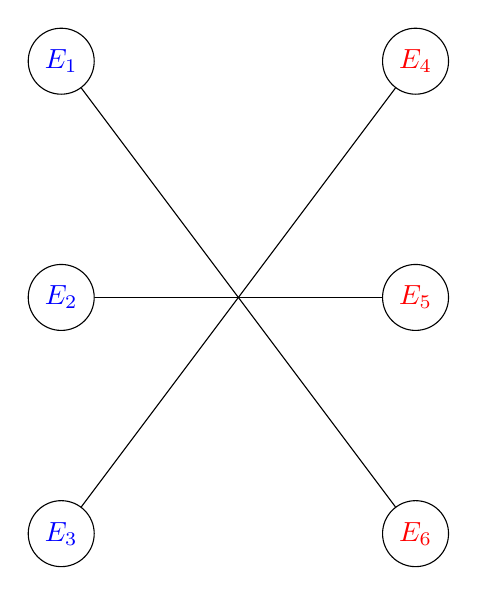
\begin{tikzpicture}[scale=3,every
	node/.style={circle,fill=white}]
      \node [draw,text=blue] (n1) at (0,3)   {$E_1$};
      \node [draw,text=blue] (n2) at (0,2)   {$E_2$};
      \node [draw,text=blue] (n3) at (0,1)   {$E_3$};
      \node [draw,text=red] (n4) at (1.5,3) {$E_4$};
      \node [draw,text=red] (n5) at (1.5,2) {$E_5$};
      \node [draw,text=red] (n6) at (1.5,1) {$E_6$};
      
      \draw [black] (n1) -- (n6);
      \draw [black] (n3) -- (n4);
      \draw [black] (n2) -- (n5);
    \end{tikzpicture}
	\caption{The access structure graph complement for a $((2,4,2))$ scheme.}
    \label{fig:2-4-2-graph}
\end{figure}

In \fref{fig:2-4-2-graph}, each vertex is an edge from \fref{fig:2-4-2}. There is an edge between the vertices if their edges are not incident to the same vertex in \fref{fig:2-4-2}. The representation illustrated in \fref{fig:2-4-2-graph} is useful to us because properties of the graph can tell us not only if a particular scheme is realizable, but why it is realizable. Let us bring in the idea of graph coloring introduced in \defref{defn:colors}.

\begin{lemma}
    \label{lem:2-color-access}
    Let a $((t,n,2))$-threshold augmented quantum secret sharing scheme have the corresponding access structure $\Gamma$. Then, this scheme is valid if and only if the access structure graph complement of $\Gamma$ is 2-colorable.
\end{lemma}

\begin{proof}
    ($\rightarrow$) Another term for 2-colorable graphs are bipartite graphs. If the AS graph of an access structure $\Gamma$ is bipartite, then we can separate the graph into two stable sets. Every pair of authorized sets in the same stable set has a non-empty intersection. So, we can assign one copy of the quantum state to each of these stable sets, and implement a QSS scheme that realizes the access structure corresponding to each particular subset of authorized sets. By construction, we have a valid augmented QTS.
    
    ($\leftarrow$) Now assume that we have a valid augmented QTS of the form $((t,n,2))$. The access structure for this scheme is $\Gamma = \Gamma_1 \cup \Gamma_2$, where $\Gamma_1$ and $\Gamma_2$ are each monotone and satisfy the no-cloning theorem. Consider just the authorized sets in $\Gamma_1$. In the AS graph complement representation, the vertices corresponding to these authorized sets must be a stable set because each pair of authorized sets in $\Gamma$ has a non-empty intersection. This is because they pairwise have a non-empty intersection. The same is true for $\Gamma_2$. Therefore, we must have a bipartite graph.
\end{proof}

By combining \lemref{lem:2-color-access} and \thmref{thm:bipartite-odd}, we get the following claim:

\begin{corollary}
    \label{cor:oddcycle-valid}
    A $((t,n,2))$ augmented QTS is valid if and only if its corresponding AS graph complement has no odd cycles.
\end{corollary}

We can use \corref{cor:oddcycle-valid} to also show that $((3,6,2))$ is also a valid scheme, but that $((2,5,2))$ and $((3,7,2))$ are \textbf{not} valid schemes.

For the $((2,5,2))$ scheme, rather than try to draw an access structure, we find an odd cycle in the AS graph complement by listing an ordering of vertices that have edges connecting them: $(1,2), (3,4), (5,1), (2,3), (4,5), (1,2)$. Each integer represents a player, and each pairing of integers represents an size-2 subset. This cycle has length 5, so the AS graph complement of $((2,5,2))$ is not bipartite. Therefore, $((2,5,2))$ does not represent a valid augmented quantum threshold scheme. A similar approach with $((3,7,2))$ leads us to the same conclusion.

From the simple cases we have studied so far, we notice a pattern beginning to emerge. It seems like schemes of the form $((t,2t,2))$ are valid, but $((t,2t+1,2))$ are not. This turns out to be true. Using the theorems that we have developed, we will formally prove these results: that all augmented QTS of the form $((t,2t,2))$ are valid, and all augmented QTS of the form $((t, 2t+1, 2))$ are not valid. Therefore, the best that we can do with two copies of a quantum secret is $((t,2t,2))$. 

\begin{remark}
    Note that if a QTS $((t,n_1))$ is not valid because it violates the no-cloning theorem, then any QTS $((t,n_2))$ where $n_2 > n_1$ can never be valid because it must also violate the no-cloning theorem. To see this, consider the QTS $((t,n_2))$. We argue that the access structure for this scheme must be a superset of the access structure for $((t,n_1))$, if $n_2 > n_1$. In fact, we can construct the smaller access structure by selecting $n_2-n_1$ players, and removing any authrozied set with which they are associated from $\Gamma_2$ to form $\Gamma_1$.
\end{remark}

\begin{theorem}
    \label{thm:t-2t-2}
    Any augmented quantum threshold scheme of the form $((t,2t,2))$ is valid using our union of access structures strategy.
\end{theorem}

\begin{proof}
    We are given an augmented quantum threshold scheme of the form $((t,2t,2))$ where $t \geq 1$. We will show that the AS graph complement of any scheme of this form is bipartite. And then, by \lemref{lem:2-color-access}, we are done. Consider one of the authorized sets, and without loss of generality, let this set have the participants: $\{p_1,\dots,p_t\}$. Then, there is only one possible authorized set that is disjoint from this one: $\{p_{t+1},\dots,p_{2t}\}$. Note that this is true for every single authorized set (of size $t$). Therefore in the AS graph complement, each vertex has degree exactly equal to 1. Such a graph must be bipartite, so $((t,2t,2))$ is valid.
\end{proof}

\begin{theorem}
    \label{thm:t-2t+1-2}
    Any augmented quantum threshold scheme of the form $((t,2t+1,2))$ is not realizable using our union of  access structures strategy.
\end{theorem}
 
\begin{proof}
    We are given an augmented quantum threshold scheme of the form $((t,2t+1,2))$ implemented over a set of players $\mathcal{P} = \{p_1,p_2,\dots,p_{2t+1}\}$, and we denote each authorized subset as an unordered set of participants. For now, assume that $t \geq 2$, because if $t=1$, the result is trivial. The only way in which we could implement a scheme over 3 players where the threshold is 1 player is to give every person a copy of the share, and we only have 2 available. 
    
    We will show that the access structure graph complement of this scheme must include an odd cycle. What we are looking for, then, is an ordered list of authorized subsets, $A_1, A_2, \dots, A_r$, such that $A_1=A_r$ and $A_i \cap A_{i+1} = \emptyset \: \forall i \in \{1,\dots,r-1\}$. If $r$ is even, then we have an odd cycle. WLOG, let the first authorized subset be $\{p_1,\dots,p_{t}\}$. From this set, we can generate a cycle of authorized sets by counting in groups of $t$ modulo $2t+1$. Here are a few of those sets in order:
    \begin{align*}
        &\{p_1,\dots,p_{t}\} \\ 
        &\{p_{t+1},\dots,p_{2t}\} \\ 
        &\{p_{2t+1},\dots,p_{t-1}\} \\ 
        &\{p_{t},\dots,p_{2t-1}\} \\
        & \vdots \\
        &\{p_{t+3},\dots,p_{1}\} \\ 
        &\{p_{2},\dots,p_{t+1}\} \\ 
        &\{p_{t+2},\dots,p_{2t+1}\} \\ 
        &\{p_1,\dots,p_{t}\}
    \end{align*}
    How many edges are in this cycle? Observe that $t$ and $2t+1$ are relatively prime, because $t \geq 2$. This means that there must be $2t+1$ edges in this cycle, which is an odd number. By \corref{cor:oddcycle-valid}, the scheme is not valid.
\end{proof}

We have shown that schemes of the form $((t,2t,2))$ are valid, but schemes of the form $((t,2t+1,2))$ are not valid. In the following chapter, we extend our results from $k=2$ to general values of $k$.





